\section{Seguimiento de carriles}

\begin{frame}\frametitle{Modelo cinemático}
  Considere la base móvil de la figura:
  \begin{figure}
    \centering
    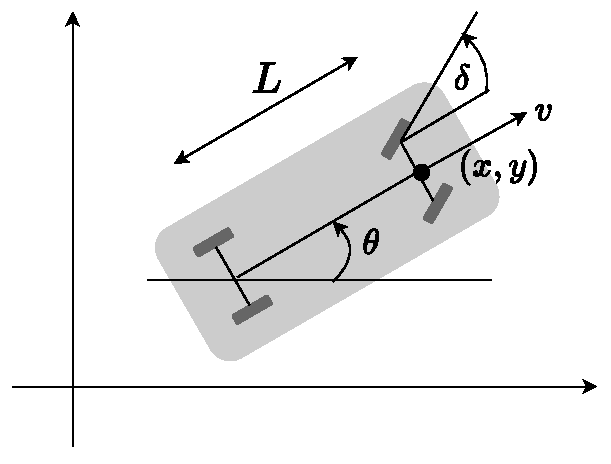
\includegraphics[width=0.3\textwidth]{Figuras/Ackermann.pdf}
  \end{figure}
  con
  \begin{itemize}
  \item $(x,y,\theta)$ la configuración en el plano de movimiento, considerando como centro el centro del eje delantero (tracción delantera)
  \item $L$ la distancia entre ejes de las llantas
  \item $v$ es la velocidad lineal del vehículo considerada como señal de entrada
  \item $\delta$ es el ángulo de las llantas delanteras (volante) también considerada como señal de control
  \end{itemize}
  El objetivo es determinar $v$ y $\delta$ de modo que le vehículo tenga determinado comportamiento.
\end{frame}

\begin{frame}\frametitle{Seguimiento de carriles}
  El seguimiento de carriles se puede hacer con base en las líneas detectadas. Considere la figura:
  
\end{frame}